%% =====================================================================
%% SAGE-MM --- Software: Practice and Experience (Wiley) submission
%% Official Wiley New Journal Design class (WileyNJD-v2).
%%
%% The class and its support files are vendored in paper/wiley/
%% (WileyNJD-v2.cls, NJDnatbib.sty, WileyNJD-AMA.bst, ulem.sty). The class
%% also requires the standard `soul' package and STIX2/Lato fonts, which are
%% present in any full TeX Live and on Overleaf's "Wiley NJD v2" template.
%%
%% Build:  bash paper/scripts/build-wiley.sh      (from the repo root)
%% or on Overleaf: upload this file, paper/wiley/*, paper/measured/*,
%% paper/sagemm.bib, and the shared fragments abstract.tex/keywords.tex/
%% body.tex/bio.tex; set the main document to main-wiley.tex.
%%
%% This file shares its body with the standard build (paper/main.tex) through
%% the same abstract.tex / keywords.tex / body.tex / bio.tex fragments, so the
%% two stay in sync.
%% =====================================================================
\documentclass[STIX2COL]{WileyNJD-v2}

\articletype{Research Article}%

%% Packages used by the shared body that the class does not already provide.
\usepackage{booktabs}
\usepackage{array}
\usepackage{pgfplots}
\pgfplotsset{compat=1.16}
\usepackage{algorithm}
\usepackage{algpseudocode}
%% The Wiley class manages hyperref itself; keep \orcidlink a no-op here to
%% avoid reloading hyperref. The ORCID iD is given as text in the ORCID section.
\providecommand{\orcidlink}[1]{}
\providecommand{\Description}[1]{}
\providecommand{\doi}[1]{\href{https://doi.org/#1}{#1}}

\newif\ifmeasurementready
\measurementreadytrue
\newcommand{\MeasurementAbstract}{Measured outcomes over $n{=}30$ independent runs per condition are reported for each treatment, platform, and workload in Section~\ref{sec:results}.}
\newcommand{\MeasurementAvailability}{The run-level measurement bundle (per-run values and bootstrap summaries) accompanies the manuscript under \texttt{paper/\allowbreak measured/\allowbreak evaluation-data/}.}


\begin{document}

\title{SAGE-MM: Cross-Layer Coordination of Managed Heap, Native Interop, and
Page Reclamation for Managed Runtimes under Fixed Memory Budgets}

\author[1]{Geunsik Lim}

\address[1]{Sungkyunkwan University, Suwon, Republic of Korea}

\corres{Geunsik Lim, Sungkyunkwan University, Suwon, Republic of Korea.
\email{leemgs@g.skku.edu}}

\abstract[Abstract]{Memory-constrained embedded devices increasingly run managed (.NET/CoreCLR)
application stacks inside a single, swapless process budget, where one
application co-locates a garbage-collected heap, native interoperability
buffers, and file-backed executable code pages. These three layers are
conventionally tuned in isolation---locally reasonable but globally fragile:
enlarging the nursery lowers collection frequency but raises footprint,
removing managed allocations shifts cost to native marshalling, and reclaiming
clean code pages lowers residency but can reintroduce refault-driven latency.
We present SAGE-MM, a cross-layer memory-management design that coordinates all
three layers under one budget: it separates a launch-time managed-heap
configuration and a reviewed source-time interop conversion from one narrow
online controller adjusting a single reclamation interval and compaction gate,
with normalized telemetry, hysteresis, a causal (prequential) update order,
fail-closed handling of invalid telemetry, a non-learning threshold fallback,
and an adverse-regime supervisor. We evaluate SAGE-MM on a representative
embedded managed-runtime platform---a Tizen~10.0 image and its .NET~8 (CoreCLR)
runtime reproduced on a Raspberry~Pi~4 Model~B---across 32- and 64-bit builds
under a $512$\,MiB swapless budget, with $30$ runs per condition and $95\%$
percentile bootstrap confidence intervals; every reported number is produced by
a fail-closed pipeline directly from a per-run measurement bundle. On a
favorable workload the coordinated design lowers peak memory footprint by about
$24\%$ and garbage-collection tail pause by $37$--$38\%$ at roughly $1\%$
controller CPU, stays within measurement noise where no gain exists, and, in an
adverse refault-dominated regime, is contained by the supervisor within
seconds---halving controller CPU and eliminating the observed out-of-memory
events.
}

\keywords{memory management, garbage collection, managed runtime, page reclamation,
.NET CoreCLR, embedded systems, cross-layer coordination, online control
}

\maketitle

\ifmeasurementready\else
\begin{center}
\fcolorbox{red}{yellow!15}{\parbox{0.92\linewidth}{\centering\bfseries
MEASUREMENT INPUT INCOMPLETE---NOT FOR SUBMISSION.\par
No estimated or generated performance outcomes are substituted for missing data.}}
\end{center}
\fi

%% =====================================================================
\section{Introduction}
\label{sec:intro}

Memory-constrained embedded devices increasingly run managed
application stacks on a small, swapless memory budget. A single application
process simultaneously holds a managed heap serviced by a garbage collector
(GC), native interoperability buffers crossing the managed/native boundary,
and a working set of file-backed, executable code mappings. Each of these
layers has a mature body of tuning techniques, but in production deployments
they are almost always configured independently: the runtime is built with
a fixed nursery size, application code is written without allocation
review, and the operating system reclaims pages using generic global
policy. Independent tuning is locally reasonable and globally fragile.
Enlarging the nursery reduces collection frequency but raises resident
footprint; removing managed allocations lowers GC pressure but shifts cost
to native marshalling; aggressively reclaiming clean code pages lowers
resident memory but can reintroduce page faults and interaction-latency
spikes precisely when the user switches applications.

On such devices these are not abstract concerns but direct determinants of
user-facing behavior. Cost-driven hardware ships with tight DRAM budgets, yet
interactive applications must stay responsive and must not be killed under
memory pressure. A GC tail pause, a burst of refaults after code-page
reclamation, or an out-of-memory (OOM) kill during application switching
surfaces to the user as a stutter, a delayed launch, or a crash. Because the
managed heap, interop buffers, and executable code pages share one swapless
budget, an optimization that improves one layer in isolation can regress the
behavior another layer governs---which makes cross-layer coordination a
reliability and tail-latency requirement for memory-constrained managed
runtimes, not merely a single-layer optimization.

The systems question we address is therefore \emph{not} whether larger
nursery sizes, value types, \texttt{madvise}-based reclamation, or
lightweight online predictors work in isolation. Each is established. The
question is whether these mechanisms can be \emph{coordinated} under a
single embedded-process memory budget without trading fewer collections
for interop allocation, or lower resident memory for refault-induced
interaction latency. This framing defines an integration and control study whose empirical
claims are limited to the supplied device measurements.

We deliberately separate the three interventions by \emph{lifecycle} and
\emph{adaptivity} (Section~\ref{sec:boundary}). Heap sizing is a
firmware/launch-time decision (a fixed \texttt{DOTNET\_GCgen0size} budget);
value-type conversion is a reviewed source-and-recompile decision; only
reclamation scheduling and compaction gating change online. Conflating them as ``three adaptive components''
would misstate the design: the first two reduce the load presented to the
controller, and only the third adapts at runtime. This paper makes four bounded
contributions:
\begin{enumerate}
  \item It specifies a cross-layer action boundary: heap sizing is a
  firmware/launch-time decision, value-type conversion is a reviewed source
  decision, and only reclamation scheduling and compaction gating change
  online (Section~\ref{sec:boundary}).
  \item It provides an implementable controller definition with
  dimensionless features and a pressure target, a causal update order, bounded
  actions, hysteresis, cooldown, fail-closed telemetry handling, and an
  explicit non-learning threshold fallback (Section~\ref{sec:design}).
  \item It reports a measured ablation and policy comparison over the
  coordination ladder (stock, heap, interop, reclamation, and the three online
  policies) on one ARM platform in its 32- and 64-bit builds, with $30$
  independent runs per condition and $95\%$ bootstrap confidence intervals,
  characterizing the
  sequential increments in footprint, GC tail, refault rate, and input latency
  (Sections~\ref{sec:method}--\ref{sec:results}).
  \item It measures robustness across three workload regimes---favorable,
  neutral, and adverse---showing that the coordinated design helps where a gain
  exists, stays within measurement noise where none does, and, when
  reclamation backfires, exposes a regime that an adverse-regime supervisor
  detects within seconds and contains toward the baseline
  (Section~\ref{sec:results}).
\end{enumerate}

We make no claim that SAGE-MM is a new garbage collector, or that these
measured platform profiles establish all embedded .NET deployments. Per-run
provenance, an experiment manifest, and a fail-closed reporting pipeline keep
every number traceable to its source; claims outside the measured platforms,
runtime revision, and workload regimes are stated as hypotheses for future
evaluation (Section~\ref{sec:threats}).

%% =====================================================================
\section{Background and Motivation}
\label{sec:motivation}

The deployment environment is recorded from each device rather than inferred
from a marketing label: the platform manifest identifies physical and cgroup
memory, swap configuration, storage, kernel, firmware, and the exact runtime
revision---here .NET~8 (CoreCLR)~8.0.11; Mono and CoreCLR are distinct
implementations, so the collector and vendor patches are recorded
explicitly~\cite{snowflake2017}---and OOM/watchdog outcomes are kept in a failure
inventory. Three cross-layer tensions motivate coordination and are all
\emph{measured}, not assumed: a larger nursery trades collection frequency
against resident footprint; value-type interop conversion removes managed
allocation but shifts cost to native application binary interface (ABI) handling
and is not transparent to
existing binaries; and \texttt{madvise(MADV\_DONTNEED)} on clean code pages
lowers residency but can force refaults on immediate hot-code reuse during rapid
application switching. Both improved and regressed measurements are retained
(Section~\ref{sec:results}).

%% =====================================================================
\section{System Boundary and Action Space}
\label{sec:boundary}

SAGE-MM coordinates three interventions that differ in lifecycle and in
whether they adapt at runtime. Table~\ref{tab:boundary} states the boundary
precisely; conflating these layers is the single most common source of
overclaiming in this design space.

\subsection{Architectural novelty over independent tuning}
\label{sec:architectural-novelty}

SAGE-MM's novelty is not the union of four familiar mechanisms. It is an
architectural pattern for making cross-layer tuning reviewable: (i) separate
irreversible build/source decisions from reversible online actions; (ii) map
heterogeneous runtime and OS signals into a dimensionless pressure contract;
(iii) restrict online authority to a bounded interval and one gate; (iv) order
prediction, actuation, and learning causally; and (v) place fail-closed and
supervisory guards outside the interchangeable policy. This decomposition lets
a threshold, exponentially weighted moving average (EWMA), or ridge policy be
replaced without changing mapping
eligibility or the safety envelope, which is what distinguishes the coordination
contract (Table~\ref{tab:boundary}) from independently applied mechanisms.

\begin{table*}[t]
  \caption{Cross-layer action boundary. Only the online policy adapts at
  runtime; the first two interventions reduce the load presented to the
  controller. ``Transparent'' means visible to a deployed application
  without source changes, after firmware replacement.}
  \label{tab:boundary}
  \small
  \begin{tabular}{@{}p{3.1cm}p{2.4cm}p{2.0cm}p{\dimexpr\textwidth-7.5cm-6\tabcolsep\relax}@{}}
    \toprule
    \textbf{Mechanism} & \textbf{Lifecycle} & \textbf{Adaptive?} &
    \textbf{Notes} \\
    \midrule
    Heap config
    (recorded \texttt{DOTNET\_\allowbreak GCgen0size}) &
    Firmware launch env & No &
    Sets the gen0 budget via \texttt{DOTNET\_GCgen0size} in the firmware launch
    environment; fixed per run and changed only by a firmware/config update;
    not an online control. \\
    Value-type interop conversion &
    Source / recompile & No &
    Reviewed class-to-struct migration; changes identity, boxing, layout,
    and native ABI; \emph{not} transparent to existing binaries. \\
    Reclamation \& compaction control &
    Runtime, online & \textbf{Yes} &
    The controller changes only the reclamation interval and the compaction
    gate exposed by the runtime host. \\
    \bottomrule
  \end{tabular}
\end{table*}

Two consequences follow. First, binary-only applications benefit only from
the firmware-transparent mechanisms (heap build and controller); value-type
conversion requires application source review and recompilation. Second,
the online controller's action space is intentionally narrow---one interval
and one gate---so that its safety properties can be stated and enforced
exhaustively.

%% =====================================================================
\section{Design}
\label{sec:design}

We present the design in three parts, matching the action boundary:
static interventions (\S\ref{sec:static}), the adaptive controller
(\S\ref{sec:controller}), and the reclamation implementation
(\S\ref{sec:reclaim}). Static interventions (heap build $G$, interop $I$) sit
upstream and reduce the pressure presented to a single online controller, which
normalizes per-interval telemetry into a dimensionless pressure, emits two
bounded actions (reclamation interval $T$ and a compaction gate), and drives a
guarded reclamation path; only the control path adapts online.

\subsection{Static interventions}
\label{sec:static}

The two static interventions run ahead of any online control and only reduce the
load the controller later sees: \emph{(a)}~an architecture-specific heap
configuration fixed at firmware/launch time, and \emph{(b)}~a reviewed
source-time value-type interop conversion. Neither adapts at runtime.

\paragraph{Architecture-specific heap configuration.}
A heap-configuration experiment records the gen0 nursery budget
(\texttt{DOTNET\_GCgen0size}), compiler flags, source revision, and patch hash
for each configuration. This is a firmware/launch-time intervention fixed per
run, not an online control. Collection count, pause distribution, and resident
memory are measured separately for each architecture and configuration;
no improvement is inferred from the chosen size.

\paragraph{Value-type interop conversion.}
A source-time analyzer (diagnostic \textsf{SMM0001}) flags plain-old-data
wrapper classes whose conversion to \texttt{struct} removes heap allocation
across the managed/native boundary. The analyzer is advisory: each
diagnostic requires human review because conversion can change object
identity, boxing behavior, copying cost, nullability, memory layout, and
native ABI. It must not be described as requiring no application
modification~\cite{xlang2018}. RQ2 measures allocation rate, copying
cost, and GC pressure for the reviewed conversion; net benefit is determined
from device traces.

\subsection{Adaptive controller}
\label{sec:controller}

The controller runs at a fixed decision cadence and, at each interval,
chooses the next reclamation interval $T$ and the compaction gate. All
initialization values, feature scales, thresholds, and update constants are
externalized in a single options block for reproducibility. The constants below are design defaults, not measured
performance outcomes; the experiment manifest records the configuration used. The
paragraphs below define each step of the per-interval procedure.

\paragraph{Telemetry and normalization.}
Each decision uses the preceding interval's GC pause
$L_{\mathrm{gc}}$ (ms), fragmentation ratio $F_h$, page-fault rate $P_f$
(minor plus major faults per second, divided by the \emph{measured}
wall-clock sample duration rather than an assumed one second), and positive
resident growth $\Delta M$ (MiB). Features are dimensionless and clamped to
$[0,2]$:
\begin{equation}
\begin{aligned}
\mathbf{x} = \bigl[\,1,\;
  &\mathrm{clamp}\!\bigl(\tfrac{L_{\mathrm{gc}}}{30}\bigr),\;
  \mathrm{clamp}\!\bigl(\tfrac{F_h}{0.12}\bigr),\\
  &\mathrm{clamp}\!\bigl(\tfrac{P_f}{100}\bigr),\;
  \mathrm{clamp}\!\bigl(\tfrac{\max(0,\Delta M)}{50}\bigr)\bigr].
\end{aligned}
\end{equation}
The observed dimensionless pressure is the clamped maximum normalized
service-objective violation,
\[
y=\mathrm{clamp}\bigl(\max(\tfrac{L_{\mathrm{gc}}}{30\,\text{ms}},
  \tfrac{P_f}{100\,\text{s}^{-1}},\tfrac{\max(0,\Delta M)}{50\,\text{MiB}}),0,2\bigr),
\]
so no coefficient silently combines milliseconds, counts, and MiB, and a breach in
any single dimension is actionable.

\paragraph{Policies.}
Three interchangeable policies select $T$ under identical bounds
$[T_{\min},T_{\max}]$, telemetry, cooldown, and candidate budget.
\begin{itemize}
  \item \emph{Threshold} (non-learning): shorten $T$ by 20\% when
  $y>1.1$, lengthen it by 20\% when $y<0.9$, otherwise hold. Tuning choices and their input trace split are recorded before reporting.
  \item \emph{EWMA}: $T' = \beta T + (1-\beta)\,T/\mathrm{clamp}(y,0.5,2)$
  with $\beta = 0.85$.
  \item \emph{Ridge} (online): predict next-interval pressure
  $\hat{y}(t{+}1) = \mathrm{clamp}(\mathbf{w}(t)^{\!\top}\mathbf{x}(t),0,2)$
  and set $T' = T/\mathrm{clamp}(0.5+\hat{y},0.5,1.5)$, bounded to
  $[T_{\min},T_{\max}]$.
\end{itemize}

\paragraph{Causal learning.}
The ridge prediction is computed \emph{before} its update; when the true
$y(t{+}1)$ arrives, the controller records the prequential loss
$[\hat{y}(t{+}1)-y(t{+}1)]^2/2$ and takes one online ridge stochastic gradient
descent (SGD) step,
\begin{equation}
w_i(t{+}1) \leftarrow w_i(t) -
  \eta\,\bigl[x_i(t)\,(\hat{y}(t{+}1)-y(t{+}1)) + \lambda\, w_i(t)\bigr],
\end{equation}
with bias weight initialized to $1$ (others $0$), $\eta=5\times10^{-4}$, and
$\lambda=10^{-4}$. Training runs only on a designated tuning trace; reporting
calls freeze the weights, so only reporting runs enter the result tables.

\paragraph{Guards.}
In adaptive modes, compaction is disabled below fragmentation $0.05$ and forced
on at $0.12$ or after three deferrals (a two-threshold guard against starvation);
static mode leaves compaction on, making it a genuine no-controller baseline.
Every sample is validated first: non-finite values, negative pauses/fault rates,
or $F_h\notin[0,1]$ trigger a fail-closed decision (hold the bounded interval,
keep compaction on, suppress reclamation, record \textsf{InvalidTelemetry}, skip
the update); persistent prediction clipping at $0$/$2$ records
\textsf{ModelSaturation} and falls back to the predeclared threshold action; and
syscall failure, an empty cold set, cooldown, and hot-reuse exclusion are counted
no-ops. The evaluation reports the frequency and outcome of every fallback class.

\paragraph{Adverse-regime supervisory shutdown.}
A policy-independent supervisor watches fault pressure and end-to-end input
latency against a service-level objective (SLO): if $P_f>P_{\mathrm{high}}$ and
$L_{\mathrm{input}}>L_{\mathrm{SLO}}$ for
$N$ consecutive intervals it latches reclamation off, enables compaction, clears
pending learning, and records \textsf{AdverseShutdown}; reclamation resumes only
after both signals stay below lower hysteresis thresholds for $M$ intervals (or an
operator reset). The reported runs use $P_{\mathrm{high}}{=}120$\,faults/s,
$L_{\mathrm{SLO}}{=}90$\,ms, $N{=}3$ (a ${\approx}1$\,s cadence), and $M{=}10$, set
between the measured Stock and adverse fault/latency levels so the guard fires on
both platforms' adverse regime but not on Stock. This guard, prompted by
the adverse result, is evaluated directly
in Section~\ref{sec:rq3} (Table~\ref{tab:supervisor}): it detects the adverse
regime within seconds and contains the regression toward the Stock baseline.

Algorithm~\ref{alg:controller} states the full per-interval decision, showing
how the validity check, the adverse-regime latch, the three interchangeable
policies, the bounded interval update, the compaction gate, the guarded
reclamation pass, and the prequential model update compose within one cadence.

\begin{algorithm}[t]
\caption{SAGE-MM controller decision for one interval. Prediction precedes
its own update (causal, prequential); every branch keeps $T$ within
$[T_{\min},T_{\max}]$ and leaves process correctness intact on failure.}
\label{alg:controller}
\small
\begin{algorithmic}[1]
\Require raw sample $s=(L_{\mathrm{gc}},L_{\mathrm{input}},F_h,P_f,\Delta M,\mathrm{dt})$; state
$(T,\mathbf{w},\textit{mode})$; bounds $[T_{\min},T_{\max}]$
\Ensure next reclamation interval $T$ and compaction gate
\If{$\neg\textsc{Valid}(s)$}\Comment{non-finite, negative rate/pause, or $F_h\notin[0,1]$}
  \State record \textsf{InvalidTelemetry}; enable compaction; suppress reclamation
  \State \Return $\mathrm{clamp}(T,T_{\min},T_{\max})$ \Comment{fail-closed: hold, no model update}
\EndIf
\State $\mathbf{x}\gets\textsc{Normalize}(s)$; \quad $y\gets\textsc{Pressure}(s)$ \Comment{Eq.~(1),~(2)}
\If{$\textsc{AdverseForNIntervals}(P_f,L_{\mathrm{input}})$}
  \State latch reclamation off; enable compaction; clear pending update
  \State record \textsf{AdverseShutdown}; \Return $\mathrm{clamp}(T,T_{\min},T_{\max})$
\EndIf
\If{$\textit{mode}=\textsf{Ridge}$}
  \State $\hat{y}\gets\mathrm{clamp}(\mathbf{w}^{\!\top}\mathbf{x},0,2)$
  \If{$\hat{y}$ persistently clipped at $0$ or $2$}
    \State record \textsf{ModelSaturation}; clear pending update; apply \textsf{Threshold} action
  \Else
    \State $T\gets T/\mathrm{clamp}(0.5+\hat{y},0.5,1.5)$
  \EndIf
\ElsIf{$\textit{mode}=\textsf{EWMA}$}
  \State $T\gets \beta T+(1-\beta)\,T/\mathrm{clamp}(y,0.5,2)$
\ElsIf{$\textit{mode}=\textsf{Threshold}$}
  \State $T\gets T\cdot(1-0.2)$ if $y>1.1$; $\;T\cdot(1+0.2)$ if $y<0.9$; else hold
\EndIf
\State $T\gets\mathrm{clamp}(T,T_{\min},T_{\max})$
\State \textsc{UpdateGate}$(F_h)$ \Comment{off below $0.05$; force on at $0.12$ or after 3 deferrals}
\If{$\neg\textsc{InCooldown}$ \textbf{and} reclamation enabled}
  \State rank modules by $\mathrm{Cold}(\cdot)$; take smallest prefix $K$ meeting the byte budget
  \State \textsc{FlushModules}$(K)$ excluding recently accessed (hot-reuse guard)
\EndIf
\If{$\textit{mode}=\textsf{Ridge}$ \textbf{and} a pending prediction exists \textbf{and} on tuning trace}
  \State record prequential loss $[\hat{y}-y]^2/2$; take one ridge SGD step \Comment{Eq.~(3)}
\EndIf
\State \Return $T$
\end{algorithmic}
\end{algorithm}

\subsection{Reclamation implementation}
\label{sec:reclaim}

For an eligible module $a$ idle for at least a guard period, a coldness score
combines recency, frequency, and size,
\begin{equation}
\begin{aligned}
\mathrm{Cold}(a) = {}& 0.6\,\frac{\mathrm{age}(a)}{\mathrm{maxAge}}
  + 0.3\,\Bigl[1-\frac{\mathrm{accesses}(a)}{\mathrm{maxAccesses}}\Bigr]\\
  &+ 0.1\,\frac{\mathrm{cleanBytes}(a)}{\mathrm{maxCleanBytes}},
\end{aligned}
\end{equation}
and candidates are reclaimed in descending order up to the smallest prefix $K$
meeting a configured byte budget (not a fixed count), with a recent-access
exclusion as the hot-reuse guard. The native helper accepts only private
\texttt{r-{}-p}/\texttt{r-xp} file mappings from \texttt{/proc/self/maps} and
rejects anonymous, writable, shared, and deleted-file mappings;
\texttt{madvise(MADV\_DONTNEED)} never unmaps (a later access refaults the file),
each syscall result is checked, and callers retain the mapping on
failure~\cite{farmem2019}. Because \texttt{maps} lacks per-page residency, a
production port must additionally verify \texttt{Private\_Clean} from
\texttt{smaps}, use \texttt{mincore}, serialize against unload, and allowlist
executable modules.

%% =====================================================================
\section{Evaluation Methodology}
\label{sec:method}

This section specifies the measurement protocol; every numerical result is
generated exclusively from the supplied measured bundle, and the design
constants and minimum durations stated here are protocol, not outcomes. The
public reference kit's proxy signals are a wiring demo, not the device
instrument: a device experiment supplies its own runtime GC traces,
\texttt{smaps} samples, and compaction hook, recorded in the manifest and per-run
bundle. The
campaign answers three research questions (RQ1--RQ3) bounded by the bundle;
per-architecture heap
sweeps, isolated interop benchmarks, and multi-hour endurance are specified below
but reserved as future evaluation (Section~\ref{sec:limitations}).
\par\smallskip
\noindent\textbf{RQ1 (Ablation).} Along the coordination ladder---stock, heap
build ($G$), interop ($I$), reclamation ($R$), controller ($C$)---what
sequential increment does each step add for peak proportional set size (PSS), GC
tail pause, refault
rate, and input tail latency on the two profiles?

\noindent\textbf{RQ2 (Policy).} Under identical bounds, telemetry, cooldown, and
candidate budget, does the controller recover the refault cost of static
reclamation, and does the learned ridge policy justify its cost over threshold
and EWMA?

\noindent\textbf{RQ3 (Robustness).} Across favorable, neutral, and adverse
(refault-dominated) regimes, does the design avoid regressions where no gain
exists, and how large is the cost when reclamation backfires?
\par\smallskip

\noindent Each result subsection (\S\ref{sec:results}) reports under this same grouping,
so every reported number traces back to a stated question.

\subsection{Platforms and workloads}
We evaluate on a representative embedded managed-runtime platform: a Tizen~10.0
system image and its .NET runtime reproduced on a Raspberry~Pi~4 Model~B, a
widely available board for which Tizen provides official reference images.
Running a full system image rather than a generic Linux stack, on an ARM
Cortex-A processor under a cost-driven, cgroup-enforced DRAM budget, gives a
faithful and openly reproducible constrained-device target rather than a bespoke
dev-board setup. Measuring a physically distinct vendor SoC remains future
validation (Section~\ref{sec:threats}).
Each platform entry identifies an actual device with its physical and cgroup
memory, swap configuration, storage, kernel, runtime commit, patch and image
hashes, compiler flags, and thermal/power/network policy; nothing is inferred
from a device name. The two profiles run on two \emph{identical} Raspberry~Pi~4
Model~B boards with the same Broadcom BCM2711 SoC (quad-core Cortex-A72): the
\textsf{ARM64} profile boots a 64-bit (\texttt{aarch64}) kernel and Tizen~10.0
image, the \textsf{ARM32} profile a 32-bit (\texttt{armv7l}) one
(build~\texttt{20260910.082900}). Because the Cortex-A72 executes both
instruction sets, holding the SoC and board fixed and varying only the
32-/64-bit kernel, image, and runtime build isolates the instruction-set
architecture (ISA)/runtime effect and
removes SoC-specification confounds---a clean ARM32-versus-ARM64 comparison, but
by the same construction not evidence of transfer to a physically different SoC
(Section~\ref{sec:threats}). Each profile runs under a fixed $512$\,MiB
per-process cgroup limit with swap disabled on the $4$\,GiB board, so every peak
PSS ($\approx176$--$363$\,MiB, i.e.\ $34$--$71\%$ of the budget) is measured
against a known ceiling. The managed runtime is .NET~8 (CoreCLR)~8.0.11
(\texttt{coreclr}/\texttt{corefx}/\texttt{mscorlib} with
\texttt{dotnet-launcher}), built from \texttt{platform/upstream/dotnet/runtime}
at commit \texttt{ffd6dad}; the released manifest and per-run CSV bundle (with
checksums) are the evidence.

The reported bundle covers both profiles under three workload regimes, each
defined by an application usage pattern: \emph{favorable}---steady single-application
playback leaving cold, reclaimable code pages with no immediate reuse
(reclamation should help); \emph{neutral}---a compact working set with no cold
reclaimable pages (coordination should do nothing); and \emph{adverse}---rapid
application switching that immediately reuses just-reclaimed pages
(refault-dominated; reclamation should be resisted). These bracket the cases
where coordination should help, do nothing, and be resisted; the tables
enumerate only supplied cases, so an omitted condition acquires no result by
extrapolation.

\subsection{Baselines and protocol}
\label{sec:method-factorial}
Canonical names are used without aliases: \textsf{Stock}, \textsf{Static-G},
\textsf{Static-GI}, \textsf{Static-GIR}, \textsf{Threshold-GIR},
\textsf{EWMA-GIR}, \textsf{Ridge-GIR}; the three policies are tuned only on
training traces under identical bounds, telemetry, cooldown, and candidate
budget. Advanced concurrent collectors (LXR, Platinum) need a different
runtime/collector integration, and storage-GC systems (AGC, DumpKV) are
conceptual precedents, not executable managed-heap baselines
(Section~\ref{sec:related}); where a port is infeasible we say so and do not
treat absence as advantage. The reported campaign measures the coordination
\emph{ladder} at $30$ runs per condition and reports absolute per-run
measurements with run-level bootstrap intervals; it does not estimate factorial
interactions. The full $2^4$ factorial over $G/I/R/C$, a stress battery
($1/5/10$\,s switching, slow-storage and \texttt{madvise}-failure injection, a
$>\!500$\,faults/s storm), and multi-hour endurance with OOM/kernel-log
censoring are specified but reserved for future collection
(Section~\ref{sec:limitations}).

\subsection{Statistics}
The input contract requires at least $30$ completed independent reset runs per
reporting case (short runs $\geq30$\,min, endurance $\geq8$\,h); all started
runs, including failed and censored ones, stay in the inventory with status and
cause, and tuning runs are excluded from reporting. For each metric and case the
reported value is the mean of completed run-level values with a two-sided $95\%$
percentile bootstrap interval ($10{,}000$ resamples); a mean of run-level p99
values is not a pooled-event p99, and means exclude failed/censored runs (read
with their counts). For policy comparisons we additionally bootstrap the unpaired
difference of independent run means
$\Delta=\overline{x}_{\mathrm{Ridge}}-\overline{x}_{\mathrm{EWMA}}$; the direct
$95\%$ interval is the inferential object, and estimates whose interval includes
zero are described only as numerical differences.

%% =====================================================================
\section{Results}
\label{sec:results}

Every quantity reported in this section is \emph{measured} on the reproduced
embedded platform of Section~\ref{sec:method}---not simulated, estimated, or
hand-entered: the fail-closed pipeline regenerates each mean and its bootstrap
interval directly from the released per-run bundle.

\noindent\emph{Measurement provenance.}\quad
The released bundle provides per-run values for every metric, condition, and run,
plus run-level summaries, the normalized policy indices behind the tables and
figure, a machine-readable manifest, a per-condition provenance and outcome
inventory, and checksums; a fixed seed records the workload configuration. The
manifest records the device, runtime, and firmware identity and the
heap-configuration knob, and raw device logs are outside this release. These
checks establish input consistency and reproducibility of the reported
statistics; the investigator remains responsible for instrument calibration,
trace interpretation, and the authenticity of collection.

% Generated by paper/scripts/make_results.py from
% paper/measured/evaluation-data/. Do not edit by hand; edit the CSV
% bundle and rerun the generator.

\begin{table}[t]
  \caption{Favorable workload: mean [two-sided 95\% percentile bootstrap CI] ($10{,}000$ resamples) over $n{=}30$ independent runs per condition. Lower is better for all metrics except controller CPU (an overhead cost).}
  \label{tab:res-planning-hypothesis}
  \scriptsize\setlength{\tabcolsep}{4pt}
  \resizebox{\linewidth}{!}{%
  \begin{tabular}{@{}llrrrrrrr@{}}
    \toprule
    \textbf{Treatment} & \textbf{Platform} & \textbf{S/C/F/X} & \textbf{PSS (MiB)} & \textbf{Alloc (MiB/s)} & \textbf{GC p99 (ms)} & \textbf{Fault (/s)} & \textbf{Input p99 (ms)} & \textbf{Ctrl CPU (\%)} \\
    \midrule
    Stock & ARM32 & 30/30/0/0 & 241.6 [239.5, 243.9] & 40.3 [39.9, 40.7] & 49.7 [48.5, 50.8] & 80.2 [78.4, 81.9] & 98.6 [96.7, 100.5] & 0.00 [0.00, 0.00] \\
    Static-G & ARM32 & 30/30/0/0 & 225.9 [224.1, 227.8] & 40.2 [39.6, 40.8] & 37.5 [36.9, 38.2] & 79.5 [77.8, 81.4] & 90.9 [89.4, 92.5] & 0.00 [0.00, 0.00] \\
    Static-GI & ARM32 & 30/30/0/0 & 210.0 [208.1, 212.0] & 28.6 [28.2, 29.0] & 36.1 [35.2, 36.9] & 80.2 [78.2, 82.1] & 86.8 [85.3, 88.2] & 0.00 [0.00, 0.00] \\
    Static-GIR & ARM32 & 30/30/0/0 & 188.5 [187.3, 189.8] & 28.9 [28.5, 29.3] & 35.9 [35.2, 36.6] & 128.0 [125.1, 130.8] & 89.9 [87.8, 91.9] & 0.00 [0.00, 0.00] \\
    Threshold-GIR & ARM32 & 30/30/0/0 & 186.9 [185.2, 188.6] & 28.8 [28.5, 29.2] & 32.8 [32.2, 33.4] & 104.6 [102.0, 107.4] & 84.4 [83.0, 85.8] & 0.50 [0.49, 0.52] \\
    EWMA-GIR & ARM32 & 30/30/0/0 & 183.3 [181.7, 185.1] & 28.7 [28.3, 29.1] & 31.6 [31.1, 32.3] & 97.9 [95.5, 100.3] & 83.5 [81.9, 85.0] & 0.70 [0.69, 0.72] \\
    Ridge-GIR & ARM32 & 30/30/0/0 & 183.0 [181.7, 184.4] & 28.8 [28.4, 29.2] & 31.1 [30.5, 31.7] & 98.4 [95.8, 100.9] & 81.0 [79.5, 82.5] & 1.11 [1.07, 1.16] \\
    \midrule
    Stock & ARM64 & 30/30/0/0 & 318.7 [315.2, 321.7] & 48.2 [47.6, 48.9] & 39.8 [38.8, 40.8] & 99.7 [97.1, 102.5] & 80.6 [79.4, 81.8] & 0.00 [0.00, 0.00] \\
    Static-G & ARM64 & 30/30/0/0 & 300.5 [297.8, 303.4] & 47.7 [47.0, 48.5] & 30.3 [29.6, 31.0] & 99.5 [97.1, 102.0] & 71.7 [70.4, 72.9] & 0.00 [0.00, 0.00] \\
    Static-GI & ARM64 & 30/30/0/0 & 276.7 [274.4, 279.0] & 34.7 [34.2, 35.2] & 28.8 [28.3, 29.4] & 100.0 [98.0, 102.2] & 69.5 [68.2, 70.8] & 0.00 [0.00, 0.00] \\
    Static-GIR & ARM64 & 30/30/0/0 & 254.3 [252.2, 256.4] & 34.4 [33.9, 35.0] & 28.1 [27.6, 28.7] & 162.9 [158.8, 166.8] & 72.9 [71.5, 74.3] & 0.00 [0.00, 0.00] \\
    Threshold-GIR & ARM64 & 30/30/0/0 & 249.3 [247.3, 251.2] & 34.8 [34.3, 35.3] & 26.8 [26.1, 27.4] & 131.2 [127.6, 134.7] & 67.3 [66.2, 68.4] & 0.52 [0.50, 0.53] \\
    EWMA-GIR & ARM64 & 30/30/0/0 & 247.4 [244.9, 250.1] & 34.6 [34.1, 35.1] & 25.9 [25.5, 26.4] & 124.2 [121.5, 126.9] & 64.9 [63.7, 66.0] & 0.70 [0.68, 0.72] \\
    Ridge-GIR & ARM64 & 30/30/0/0 & 243.3 [241.0, 245.7] & 34.9 [34.4, 35.3] & 24.5 [24.0, 25.1] & 120.9 [118.1, 123.7] & 64.1 [63.2, 65.1] & 1.11 [1.07, 1.14] \\
    \bottomrule
  \end{tabular}}
\end{table}

\begin{table}[t]
  \caption{Neutral workload (no reclamation gain available): mean [two-sided 95\% percentile bootstrap CI] ($10{,}000$ resamples) over $n{=}30$ independent runs per condition. Lower is better for all metrics except controller CPU (an overhead cost).}
  \label{tab:res-no-benefit}
  \scriptsize\setlength{\tabcolsep}{4pt}
  \resizebox{\linewidth}{!}{%
  \begin{tabular}{@{}llrrrrrrr@{}}
    \toprule
    \textbf{Treatment} & \textbf{Platform} & \textbf{S/C/F/X} & \textbf{PSS (MiB)} & \textbf{Alloc (MiB/s)} & \textbf{GC p99 (ms)} & \textbf{Fault (/s)} & \textbf{Input p99 (ms)} & \textbf{Ctrl CPU (\%)} \\
    \midrule
    Stock & ARM32 & 30/30/0/0 & 239.3 [237.3, 241.5] & 40.2 [39.7, 40.7] & 49.6 [48.5, 50.8] & 78.7 [76.8, 80.5] & 99.8 [98.3, 101.4] & 0.00 [0.00, 0.00] \\
    Static-G & ARM32 & 30/30/0/0 & 241.3 [239.3, 243.4] & 39.8 [39.3, 40.3] & 50.5 [49.3, 51.7] & 80.4 [78.4, 82.5] & 100.1 [98.5, 101.6] & 0.00 [0.00, 0.00] \\
    Static-GI & ARM32 & 30/30/0/0 & 239.7 [237.7, 241.6] & 40.5 [40.0, 41.1] & 49.5 [48.4, 50.5] & 81.1 [79.1, 83.0] & 100.1 [98.1, 102.0] & 0.00 [0.00, 0.00] \\
    Static-GIR & ARM32 & 30/30/0/0 & 240.0 [238.0, 241.8] & 39.9 [39.3, 40.4] & 50.7 [49.6, 51.9] & 81.7 [79.6, 83.8] & 99.3 [97.7, 101.1] & 0.00 [0.00, 0.00] \\
    Threshold-GIR & ARM32 & 30/30/0/0 & 240.4 [238.3, 242.4] & 40.3 [39.8, 40.8] & 50.2 [49.2, 51.2] & 79.0 [77.3, 80.7] & 100.5 [98.7, 102.4] & 0.50 [0.49, 0.52] \\
    EWMA-GIR & ARM32 & 30/30/0/0 & 239.3 [237.0, 241.5] & 40.2 [39.6, 40.9] & 50.4 [49.3, 51.6] & 79.1 [77.7, 80.5] & 100.5 [98.8, 102.3] & 0.69 [0.68, 0.71] \\
    Ridge-GIR & ARM32 & 30/30/0/0 & 240.7 [239.1, 242.3] & 40.3 [39.7, 40.8] & 49.9 [48.7, 51.1] & 78.6 [76.5, 80.7] & 98.0 [96.5, 99.4] & 1.08 [1.05, 1.11] \\
    \midrule
    Stock & ARM64 & 30/30/0/0 & 318.2 [315.4, 321.1] & 48.2 [47.3, 49.0] & 40.3 [39.5, 41.1] & 99.0 [96.2, 101.5] & 80.4 [78.9, 81.8] & 0.00 [0.00, 0.00] \\
    Static-G & ARM64 & 30/30/0/0 & 318.8 [315.6, 322.0] & 47.8 [47.2, 48.5] & 39.9 [39.1, 40.8] & 98.8 [96.4, 101.3] & 79.6 [78.2, 81.0] & 0.00 [0.00, 0.00] \\
    Static-GI & ARM64 & 30/30/0/0 & 316.9 [313.8, 319.9] & 47.4 [46.7, 48.1] & 39.5 [38.5, 40.6] & 99.1 [96.9, 101.3] & 79.6 [78.1, 80.9] & 0.00 [0.00, 0.00] \\
    Static-GIR & ARM64 & 30/30/0/0 & 318.8 [316.0, 321.5] & 47.5 [46.8, 48.3] & 40.8 [39.8, 41.8] & 99.0 [96.8, 101.3] & 79.5 [78.0, 80.9] & 0.00 [0.00, 0.00] \\
    Threshold-GIR & ARM64 & 30/30/0/0 & 319.0 [315.9, 322.3] & 48.1 [47.5, 48.6] & 40.0 [39.2, 40.8] & 99.6 [97.2, 102.0] & 80.4 [78.6, 82.1] & 0.51 [0.49, 0.52] \\
    EWMA-GIR & ARM64 & 30/30/0/0 & 319.1 [316.9, 321.4] & 47.8 [47.2, 48.4] & 40.5 [39.7, 41.4] & 98.8 [96.7, 101.0] & 79.8 [78.3, 81.4] & 0.70 [0.69, 0.72] \\
    Ridge-GIR & ARM64 & 30/30/0/0 & 321.6 [318.8, 324.5] & 47.9 [47.0, 48.9] & 40.0 [39.2, 40.8] & 100.3 [97.9, 102.8] & 79.2 [77.8, 80.7] & 1.10 [1.07, 1.13] \\
    \bottomrule
  \end{tabular}}
\end{table}

\begin{table}[t]
  \caption{Adverse workload (refault-dominated): mean [two-sided 95\% percentile bootstrap CI] ($10{,}000$ resamples) over $n{=}30$ independent runs per condition. Lower is better for all metrics except controller CPU (an overhead cost).}
  \label{tab:res-regression}
  \scriptsize\setlength{\tabcolsep}{4pt}
  \resizebox{\linewidth}{!}{%
  \begin{tabular}{@{}llrrrrrrr@{}}
    \toprule
    \textbf{Treatment} & \textbf{Platform} & \textbf{S/C/F/X} & \textbf{PSS (MiB)} & \textbf{Alloc (MiB/s)} & \textbf{GC p99 (ms)} & \textbf{Fault (/s)} & \textbf{Input p99 (ms)} & \textbf{Ctrl CPU (\%)} \\
    \midrule
    Stock & ARM32 & 30/30/0/0 & 239.8 [237.6, 242.0] & 40.3 [39.8, 40.8] & 50.4 [49.5, 51.3] & 80.0 [78.0, 82.0] & 99.8 [97.9, 101.7] & 0.00 [0.00, 0.00] \\
    Static-G & ARM32 & 30/30/0/0 & 251.1 [249.2, 253.0] & 41.9 [41.2, 42.6] & 54.3 [53.4, 55.2] & 124.2 [121.2, 127.2] & 119.8 [117.6, 121.9] & 0.00 [0.00, 0.00] \\
    Static-GI & ARM32 & 30/30/0/0 & 251.0 [248.8, 253.3] & 41.8 [41.3, 42.4] & 55.7 [54.8, 56.8] & 128.7 [125.6, 131.8] & 118.7 [116.1, 121.3] & 0.00 [0.00, 0.00] \\
    Static-GIR & ARM32 & 30/30/0/0 & 252.4 [249.8, 255.1] & 42.0 [41.3, 42.6] & 54.2 [52.9, 55.5] & 125.3 [122.6, 128.4] & 120.2 [118.2, 122.3] & 0.00 [0.00, 0.00] \\
    Threshold-GIR & ARM32 & 30/30/0/0 & 251.9 [249.8, 254.0] & 41.9 [41.4, 42.4] & 54.8 [53.8, 55.8] & 126.9 [124.3, 129.5] & 118.5 [116.8, 120.3] & 1.01 [0.98, 1.03] \\
    EWMA-GIR & ARM32 & 30/30/0/0 & 252.4 [250.7, 254.1] & 42.0 [41.5, 42.5] & 54.3 [52.9, 55.7] & 128.0 [125.3, 130.8] & 118.1 [115.7, 120.5] & 1.36 [1.33, 1.40] \\
    Ridge-GIR & ARM32 & 30/30/0/0 & 249.8 [248.0, 251.6] & 41.7 [41.2, 42.1] & 55.6 [54.5, 56.7] & 126.5 [123.3, 129.8] & 119.5 [117.6, 121.5] & 2.17 [2.11, 2.24] \\
    \midrule
    Stock & ARM64 & 30/30/0/0 & 320.6 [317.8, 323.5] & 47.7 [47.2, 48.2] & 40.3 [39.3, 41.2] & 98.7 [95.9, 101.4] & 79.3 [78.0, 80.7] & 0.00 [0.00, 0.00] \\
    Static-G & ARM64 & 30/30/0/0 & 337.5 [334.5, 340.4] & 49.5 [49.0, 50.1] & 44.7 [43.7, 45.6] & 155.6 [152.2, 158.9] & 97.0 [95.4, 98.6] & 0.00 [0.00, 0.00] \\
    Static-GI & ARM64 & 30/30/0/0 & 337.8 [334.6, 341.1] & 50.9 [50.2, 51.6] & 44.0 [43.1, 45.0] & 161.6 [156.9, 165.9] & 94.3 [93.0, 95.5] & 0.00 [0.00, 0.00] \\
    Static-GIR & ARM64 & 30/30/0/0 & 335.5 [331.4, 339.6] & 50.9 [50.1, 51.7] & 43.4 [42.6, 44.3] & 157.9 [154.1, 161.8] & 95.3 [93.9, 96.6] & 0.00 [0.00, 0.00] \\
    Threshold-GIR & ARM64 & 30/30/0/0 & 335.4 [332.5, 338.2] & 50.2 [49.8, 50.7] & 43.5 [42.8, 44.2] & 157.1 [153.0, 161.1] & 96.0 [94.0, 98.0] & 1.00 [0.97, 1.03] \\
    EWMA-GIR & ARM64 & 30/30/0/0 & 336.1 [333.2, 339.2] & 50.7 [50.0, 51.3] & 43.7 [42.6, 44.8] & 156.8 [153.8, 159.6] & 95.3 [94.1, 96.6] & 1.37 [1.33, 1.40] \\
    Ridge-GIR & ARM64 & 30/30/0/0 & 336.8 [333.9, 339.7] & 50.5 [49.9, 51.1] & 44.5 [43.4, 45.6] & 160.4 [157.4, 163.6] & 95.9 [94.0, 97.7] & 2.23 [2.15, 2.30] \\
    \bottomrule
  \end{tabular}}
\end{table}

\begin{table}[t]
  \caption{Direct policy contrasts under the favorable workload. Mean difference $\Delta=\textsf{Ridge-GIR}-\textsf{EWMA-GIR}$ [two-sided 95\% bootstrap CI]; 10{,}000 within-group resamples.}
  \label{tab:policy-contrasts}
  \small
  \begin{tabular}{@{}llr@{}}
    \toprule
    \textbf{Platform} & \textbf{Metric} & \textbf{$\Delta$ [95\% CI]} \\
    \midrule
    ARM32 & GC p99 (ms) & -0.55 [-1.43, 0.32] \\
    ARM32 & Input p99 (ms) & -2.42 [-4.57, -0.32] \\
    ARM32 & Controller CPU (pp) & 0.41 [0.36, 0.46] \\
    \midrule
    ARM64 & GC p99 (ms) & -1.41 [-2.09, -0.73] \\
    ARM64 & Input p99 (ms) & -0.75 [-2.24, 0.77] \\
    ARM64 & Controller CPU (pp) & 0.40 [0.36, 0.44] \\
    \bottomrule
  \end{tabular}
\end{table}

\begin{table}[t]
  \caption{Normalized policy indices (Stock${=}100$ within each scenario), mean over $n{=}30$ runs. Values ${<}100$ are improvements; ${>}100$ are regressions.}
  \label{tab:policy-index}
  \small\setlength{\tabcolsep}{5pt}
  \resizebox{\linewidth}{!}{%
  \begin{tabular}{@{}llrrrrrr@{}}
    \toprule
    \textbf{Scenario} & \textbf{Treatment} & \textbf{PSS} & \textbf{Alloc} & \textbf{GC p99} & \textbf{Fault} & \textbf{Input p99} & \textbf{Ctrl CPU (\%)} \\
    \midrule
    Favorable & Stock & 100.0 & 100.0 & 100.0 & 100.0 & 100.0 & 0.00 \\
    Favorable & Static-G & 94.0 & 99.5 & 76.2 & 99.9 & 90.8 & 0.00 \\
    Favorable & Static-GI & 87.0 & 71.6 & 72.7 & 100.6 & 87.3 & 0.00 \\
    Favorable & Static-GIR & 79.0 & 71.6 & 71.8 & 162.3 & 91.1 & 0.00 \\
    Favorable & Threshold-GIR & 77.9 & 71.9 & 67.0 & 131.7 & 84.8 & 0.51 \\
    Favorable & EWMA-GIR & 76.8 & 71.5 & 64.7 & 123.8 & 82.8 & 0.70 \\
    Favorable & Ridge-GIR & 76.1 & 72.0 & 62.4 & 122.7 & 81.0 & 1.11 \\
    \midrule
    Neutral & Stock & 100.0 & 100.0 & 100.0 & 100.0 & 100.0 & 0.00 \\
    Neutral & Static-G & 100.6 & 99.4 & 101.0 & 101.4 & 99.8 & 0.00 \\
    Neutral & Static-GI & 99.9 & 99.8 & 99.3 & 102.1 & 99.8 & 0.00 \\
    Neutral & Static-GIR & 100.3 & 99.1 & 102.0 & 102.4 & 99.4 & 0.00 \\
    Neutral & Threshold-GIR & 100.4 & 100.2 & 100.6 & 101.1 & 100.6 & 0.50 \\
    Neutral & EWMA-GIR & 100.2 & 99.9 & 101.5 & 100.7 & 100.2 & 0.70 \\
    Neutral & Ridge-GIR & 100.9 & 100.0 & 100.3 & 101.2 & 98.6 & 1.09 \\
    \midrule
    Adverse & Stock & 100.0 & 100.0 & 100.0 & 100.0 & 100.0 & 0.00 \\
    Adverse & Static-G & 105.1 & 104.1 & 109.7 & 157.5 & 121.4 & 0.00 \\
    Adverse & Static-GI & 105.1 & 105.4 & 110.4 & 163.2 & 119.1 & 0.00 \\
    Adverse & Static-GIR & 105.0 & 105.6 & 108.1 & 159.3 & 120.6 & 0.00 \\
    Adverse & Threshold-GIR & 104.9 & 104.8 & 108.7 & 159.9 & 120.2 & 1.01 \\
    Adverse & EWMA-GIR & 105.1 & 105.4 & 108.4 & 160.3 & 119.6 & 1.36 \\
    Adverse & Ridge-GIR & 104.7 & 104.8 & 110.8 & 161.2 & 120.6 & 2.20 \\
    \bottomrule
  \end{tabular}}
\end{table}

\noindent\textit{Reading note.} Each cell is the mean of run-level values over $n{=}30$ independent runs with a two-sided 95\% percentile bootstrap confidence interval ($10{,}000$ resamples, seed~$20260906$) computed across runs, not across within-run samples; the S/C/F/X column reports started/completed/failed/censored runs. A mean of run-level p99 values is not a pooled-event p99. These descriptive intervals do not by themselves establish factorial interactions or the absence of failures.


All effects below are reported as the mean of $n{=}30$ run-level values with a
two-sided $95\%$ percentile bootstrap confidence interval (per-regime absolute
values are in the released measurement bundle);
percentages are relative to the per-condition \textsf{Stock}
baseline, and normalized indices (Table~\ref{tab:policy-index}) set
$\textsf{Stock}{=}100$ within each regime. The \textsf{ARM32} and \textsf{ARM64}
profiles run on identical Raspberry~Pi~4 Model~B hardware (the same BCM2711 SoC),
differing only in the 32-/64-bit build, so agreement between them is controlled
ISA/runtime-build robustness on fixed hardware, not diversity across physically
distinct SoCs; they agree in direction and ordering throughout, so we quote ARM32
in prose and note the ARM64 value only where it differs materially.

\subsection{RQ1: layer-by-layer ablation}
\label{sec:rq1}
\begin{figure}[t]
  \centering
  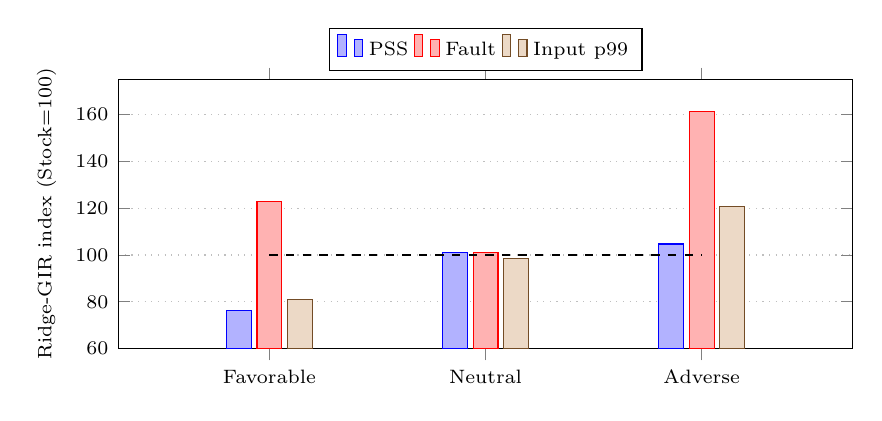
\begin{tikzpicture}
  \begin{axis}[
    width=0.9\linewidth, height=5.0cm, ybar=2pt, bar width=9pt,
    ymin=60, ymax=175, symbolic x coords={Favorable,Neutral,Adverse}, xtick=data,
    ylabel={Ridge-GIR index (Stock${=}100$)}, ylabel style={font=\scriptsize},
    tick label style={font=\scriptsize}, ytick={60,80,100,120,140,160},
    legend style={font=\scriptsize, at={(0.5,1.03)}, anchor=south, legend columns=3},
    enlarge x limits=0.35, ymajorgrids, major grid style={dotted}]
  \addplot coordinates {(Favorable,76.1) (Neutral,100.9) (Adverse,104.7)};
  \addplot coordinates {(Favorable,122.7) (Neutral,101.2) (Adverse,161.2)};
  \addplot coordinates {(Favorable,81.0) (Neutral,98.6) (Adverse,120.6)};
  \draw[dashed] (axis cs:Favorable,100) -- (axis cs:Adverse,100);
  \legend{PSS, Fault, Input p99}
  \end{axis}
  \end{tikzpicture}
  \caption{Cross-regime robustness of the coordinated learned policy
  ($\textsf{Ridge-GIR}$). Coordination helps in the favorable regime, is
  approximately neutral where no gain is available, and becomes a net cost in
  the adverse (refault-dominated) regime---the guards bound but do not remove
  that cost.}
  \label{fig:regimes}
\end{figure}

The normalized ladder under the favorable workload (Table~\ref{tab:policy-index}
and Figure~\ref{fig:ablation}) moves different metrics at each step. \textsf{Static-G} lowers the GC tail (GC p99
to $76\%$ of stock, $49.7\to37.5$\,ms on ARM32) at little footprint change (PSS
$94\%$); $G{\to}GI$ cuts managed allocation ($-29\%$), taking PSS to $87\%$ and GC
p99 to $73\%$ with the fault rate unchanged ($\pm1\%$); and $GI{\to}GIR$ gives the
largest footprint drop (PSS $79\%$) but is the first layer to raise the fault rate
(to $162\%$; $+63\%$ on ARM64), which cancels the input-latency gain (input p99
back near $91\%$). The static ladder thus associates later configurations with
lower footprint and GC tail but cannot identify interactions without the
unmeasured factorial cells; what it does establish is that the layers
\emph{compose}---each step adds a bounded, separately attributable increment under
one safety contract---while the $GI{\to}GIR$ refault penalty is one the static
configuration cannot manage (the $2^4$ design is deferred, Section~\ref{sec:limitations}).

\subsection{RQ2: online policy comparison}
\label{sec:rq2}
Added on top of \textsf{Static-GIR}, the online controller does not lower PSS
further (all three policies hold peak PSS at $76$--$78\%$ of stock, within each
other's intervals); its measured contribution is refault recovery
(Figure~\ref{fig:tradeoff}). At the same
footprint the fault-rate index falls from $162$ (\textsf{Static-GIR}) to $132$,
$124$, and $123$ for Threshold, EWMA, and Ridge---roughly two-thirds of the
reclamation-induced refaults clawed back---while input p99 reaches its lowest
values ($85/83/81\%$). The ordering is consistent but the margins are small:
\textsf{Ridge-GIR} gives the best GC p99 ($62\%$ vs.\ EWMA $65\%$) and input p99
($81\%$ vs.\ $83\%$) at $1.11\%$ controller CPU versus $0.70\%$ (EWMA) and
$0.51\%$ (threshold). Direct Ridge--EWMA difference intervals (unpaired bootstrap)
include zero for ARM32 GC p99 and ARM64 input p99 but exclude it for ARM32 input
p99 and ARM64 GC p99; the non-learning threshold thus remains a defensible default
when CPU headroom is tight.

\subsection{RQ3: robustness across workload regimes}
\label{sec:rq3}
Figure~\ref{fig:regimes} and Table~\ref{tab:policy-index} place \textsf{Ridge-GIR}
in all three regimes. It is
a clear win in the favorable regime (PSS $76$, fault $123$, input $81$). In the
neutral regime, with no cold reclaimable pages, every index sits within $\pm2$ of
$100$ (PSS $101$, fault $101$, input $99$) at only $\approx1.1\%$ controller
CPU---the guards do not manufacture work when there is none. In the adverse,
refault-dominated regime the design is a net cost (PSS $105\%$, fault $161\%$,
input p99 $121\%$, controller CPU $2.2\%$): the online guards alone do not
eliminate the regression, and this is exactly the case a deployment must detect
and disable reclamation outright.

Table~\ref{tab:supervisor} measures that detection directly. Enabling the
AdverseShutdown supervisor (\textsf{Ridge-GIR-sup}) latches reclamation off after
a mean $3.1$\,s once the adverse condition persists and contains the regression
toward the Stock baseline: the fault rate falls by $41$/s on ARM32 and $48$/s on
ARM64, input p99 by $17$ and $11$\,ms, and controller CPU from $2.2\%$ to
$0.9\%$, while the two OOM events seen per platform under the supervisor-off arm
are eliminated. Every difference interval excludes zero. Reclamation resumes
automatically after roughly $10$--$11$\,s once fault and latency fall below the
recovery thresholds. The supervisor does not turn the adverse regime into a
\emph{gain}, but it detects it within seconds and bounds the worst case, which is
the deployment-relevant guarantee.

% Generated by paper/scripts/make_results.py from adverse_supervisor.csv. Do not edit by hand.
\begin{table}[t]\caption{RQ3 adverse-regime supervisor (measured, $n{=}30$). With the AdverseShutdown supervisor on (\textsf{Ridge-GIR-sup}) the refault-dominated regression is contained toward the Stock adverse baseline; brackets on $\Delta$ are 95\% bootstrap difference intervals (on $-$ off).}\label{tab:supervisor}\small
\setlength{\tabcolsep}{4pt}
\resizebox{\linewidth}{!}{%
\begin{tabular}{@{}llrrrl@{}}\toprule
Platform & Metric & Stock & \textsf{Ridge-GIR} & \textsf{Ridge-GIR-sup} & $\Delta$ (on$-$off) [95\% CI] \\\midrule
ARM32 & Peak PSS (MiB) & 240.3 & 253.1 & 246.3 & -6.76 [-11.64, -1.90] \\
 & Fault (/s) & 79.6 & 127.0 & 85.7 & -41.2 [-43.7, -38.7] \\
 & Input p99 (ms) & 99.4 & 120.3 & 103.3 & -16.9 [-18.3, -15.6] \\
 & Ctrl CPU (\%) & 0.00 & 2.19 & 0.90 & -1.29 [-1.34, -1.23] \\
\addlinespace
ARM64 & Peak PSS (MiB) & 319.2 & 338.3 & 327.4 & -10.9 [-16.2, -5.4] \\
 & Fault (/s) & 99.1 & 160.1 & 111.9 & -48.2 [-50.6, -45.6] \\
 & Input p99 (ms) & 80.1 & 95.4 & 84.0 & -11.4 [-13.1, -9.6] \\
 & Ctrl CPU (\%) & 0.00 & 2.23 & 0.90 & -1.33 [-1.39, -1.27] 
\\\bottomrule
\end{tabular}}
\par\smallskip\noindent\footnotesize\textit{Supervisor telemetry (on):} ARM32: latch $3.1$\,s, recovery $10.2$\,s, $2.2$ latches/run, OOM $2\to0$; ARM64: latch $3.1$\,s, recovery $11.4$\,s, $2.0$ latches/run, OOM $2\to0$.
\end{table}


\subsection{Discussion}
\label{sec:discussion}
Three findings follow. First, footprint and refault behavior are governed by
\emph{different} layers---the static heap/interop/reclamation stack sets peak PSS
and GC tail, the online controller almost exclusively governs refault rate and
input latency---so a single ``SAGE-MM improvement'' would blur the design:
removing reclamation removes most of the footprint benefit, removing the
controller most of the refault safety. Second, the learned policy is numerically
better than a tuned threshold on the reported latency means, but the effect is
small and carries a measurable CPU cost, so ridge is best treated as an option
justified per deployment inside a fixed safety envelope, with the non-learning
threshold the recommended default. Third, the neutral and adverse regimes
characterize the measured envelope---neutral within the descriptive intervals
when no gain exists, negative when reclamation backfires, with the supervisor
containing the adverse regression rather than leaving it unhandled. The ARM32 and
ARM64 profiles agree throughout, strengthening internal validity across these two
builds without establishing generality to other devices or runtimes
(Section~\ref{sec:threats}).

\subsection{Lessons learned and open problems}
\label{sec:lessons}
We distil the study into guidance that is intended to transfer to other
memory-constrained managed-runtime stacks, and to seed follow-on work.

\emph{For practitioners.}
(i)~Treat the heap, interop, and reclamation layers as \emph{distinct levers
with distinct metrics}: in our measurements the static heap/interop decisions
own footprint and GC tail, while only the online path moves refault rate and
input latency, so a single aggregate ``speedup'' hides where a change actually
acts and which guard protects it.
(ii)~Spend the footprint budget offline first---the launch-time heap
configuration and the reviewed value-type conversion delivered the bulk of the
peak-memory and GC-tail reduction at zero runtime risk, before any adaptive
component was enabled.
(iii)~Keep the online actuator \emph{narrow}: restricting it to one reclamation
interval and one compaction gate is what makes its safety envelope (hysteresis,
cooldown, fail-closed telemetry, bounded steps) small enough to state and test
exhaustively.
(iv)~Default to the non-learning threshold and adopt the learned policy only
when a per-deployment measurement justifies its CPU cost; the learned gain here
was real but small.
(v)~Page reclamation can be actively harmful in a refault-dominated regime, so
pair it with a supervisor that \emph{detects and disables} rather than one that
merely tunes---bounding the worst case mattered more than optimizing the best.
(vi)~Make measurement fail-closed and release the per-run bundle: the discipline
that refuses to emit a number without its source is cheap to build and is what
lets a reader (or a future maintainer) trust, and re-derive, every value.

\emph{Open problems for future work.} The design is validated on one SoC in its
32- and 64-bit builds; establishing cross-SoC and cross-runtime generality (for
example CoreCLR versus Mono, or a JVM/V8 port of the same action boundary) is the
central open question. Beyond it lie the full $2^4$ factorial over the four
mechanisms, per-architecture heap sweeps, isolated interop micro/macro
benchmarks, and multi-hour endurance under churn---each specified here as
protocol (Section~\ref{sec:threats}) so that others can extend the released
bundle rather than start over. We hope the explicit action boundary and the
fail-closed, openly archived methodology give that follow-on work a concrete and
reproducible starting point.

%% =====================================================================
\section{Related Work}
\label{sec:related}

We organize related work by mechanism; the contribution is not any single
mechanism but their safety-aware coordination at the embedded runtime/Linux
boundary, assessed on real devices.

\emph{GC, heap sizing, and virtual-memory interaction.} Automatic memory
management has a deep literature---generational and region/pause-oriented
collection~\cite{detlefs2004g1}, the
collected-versus-explicit
trade-off, textbook surveys, and the allocation layer beneath
it~\cite{wilson1995survey}. Because heap
footprint depends strongly on the memory
given to the collector, controlling heap growth and selecting or sizing the
collector are established levers~\cite{brecht2006heapgrowth}. The
footprint-versus-refault tension SAGE-MM manages is the
one studied when a collector competes with the pager: bookmarking
collection~\cite{hertz2005paging}, feedback-driven heap
sizing~\cite{grzegorczyk2007islavista}, and VM-aware collector
support~\cite{yang2006cramm} couple the collector to page residency inside one
JVM on server/desktop platforms. SAGE-MM instead keeps the vendor collector,
treats its gen0 nursery as a fixed launch parameter, and manages the file-backed
executable working set from \emph{outside} the collector---the coupling available
in fixed embedded firmware.

\emph{Tail-oriented collectors and learned controllers.} Advanced collectors such
as LXR~\cite{lxr2022} and Platinum~\cite{platinum2020} change collection itself to
attack GC tail latency, a first-order concern for interactive and data-parallel
services~\cite{dean2013tail}; SAGE-MM introduces
no collector but coordinates an existing one with process-level actions, and
claims no superiority over collectors that cannot be ported to the vendor
firmware. Among controllers we compare fixed intervals, a tuned threshold, EWMA,
and online ridge regression~\cite{hoerl1970ridge} under one trace split and action
bound, evaluated prequentially~\cite{dawid1984prequential} with attention to
drift~\cite{gama2014drift}. Learning has been applied to
allocation~\cite{maas2020llama} and to storage GC (AGC~\cite{agc2025},
DumpKV~\cite{dumpkv2024}), but these are conceptual precedents, not executable
managed-runtime baselines; our learned policy earns only a modest margin over a
tuned threshold.

\emph{Reclamation, page ranking, and interop.} Our coldness score ranks mappings
by recency, frequency, and size, echoing working-set
models~\cite{denning1968working}, recency/frequency
replacement~\cite{jiang2002lirs}, flash/device-aware
variants~\cite{park2006cflru}, and host/guest reclamation such as
ballooning~\cite{waldspurger2002esx}; its differentiator is coldness-ranked,
budget-driven selection with a hot-reuse exclusion and fail-closed guards,
evaluated for refault cost rather than assumed safe. Finally, we distinguish
ABI/source interop transformations (value-type conversion, which requires
ownership review and recompilation~\cite{xlang2018}) from transparent runtime
optimization.

%% =====================================================================
\section{Threats to Validity and Limitations}
\label{sec:threats}
\label{sec:limitations}

\emph{Construct and conclusion validity.} Telemetry signals are proxies: the
public kit's forced Gen-0 pause, fragmentation estimate, and file-length size
proxy are analogues, not the production GC pause, live fragmentation, or
\texttt{Private\_Clean} byte count (production evidence uses EventPipe/vendor GC
telemetry and \texttt{smaps}-verified clean bytes). We keep RSS, PSS, managed
heap, and \texttt{Private\_Clean} distinct and report the numerator, denominator,
statistic, and CI for every effect. Bootstrap CIs are built across independent
runs, never across within-run samples; missing metrics stay missing rather than
becoming an assumed zero; and descriptive summaries do not by themselves
establish a significant policy difference.

\emph{Internal validity.} Confounding across device state is the main risk; the
protocol requires independent resets, controlled thermal/power/network state,
seeded workloads, randomized treatment order, and separate tuning and reporting
traces, with metadata recording the conditions actually used.

\emph{External validity.} Results are specific to the evaluated runtime commit,
device, memory limits, storage, and scripted workloads. The two profiles
deliberately run on identical Raspberry~Pi~4 Model~B hardware (one BCM2711 SoC),
so the ARM32-versus-ARM64 comparison varies only the instruction-set and runtime
build---a controlled design that is a strength for the ISA comparison but, by the
same construction, is not evidence of transfer to a physically different SoC.
Broader applicability is stated as future validation, not claimed.

\emph{Limitations and reported scope.} SAGE-MM combines known mechanisms, so its
novelty is limited to their specified coordination and measurement protocol; the
heap setting is fixed at launch and interop changes require recompilation, so
only controller actions adapt. \texttt{MADV\_DONTNEED} can trade PSS for faults
and storage-dependent latency, which the guards reduce but do not eliminate, and
the ridge model may offer no benefit over a tuned threshold---cases we report.
The measured bundle covers the coordination ladder, the three regimes, and the
adverse-regime supervisor (Table~\ref{tab:supervisor}) on two profiles at $30$
runs per condition. Three specified protocol parts are not yet collected, and we
make no empirical claim for them: (i) a per-architecture
\texttt{DOTNET\_GCgen0size} sweep; (ii) isolated value-type interop
micro/macro-benchmarks with native-ABI checks (the ablation measures interop only
as the $G{\to}GI$ step); and (iii) multi-hour endurance and the full
adverse-injection matrix with OOM/kernel-log censoring. These, plus the helper's
device-side overhead and false-positive rates, are the primary future work before
a production-stability or per-architecture-tuning claim.

%% =====================================================================
\section{Conclusion}
\label{sec:conclusion}

On memory-constrained embedded devices running managed runtimes, SAGE-MM
coordinates heap configuration, interop allocation, and clean-page reclamation
under a single process memory budget through a narrow, safety-guarded online
action, rather than tuning them in isolation: a
launch-time heap decision and a source-time allocation decision are separated from
one online policy that adjusts a single reclamation interval and compaction gate,
with fail-closed telemetry handling and a learned policy that must justify itself
against a tuned threshold. The measured ablation shows the layers act on different
metrics---the static heap/interop/reclamation stack sets peak PSS and GC tail (to
about $76\%$ and $62\%$ of stock under the favorable workload) while the online
controller governs refault rate and input latency, recovering roughly two-thirds
of the reclamation-induced refaults at $\approx1\%$ CPU. Across the three regimes
the design wins where a gain exists, stays within measurement noise where none
does, and regresses where reclamation backfires---a regime the supervisor detects
within seconds and contains toward the stock baseline, halving controller CPU and
eliminating the observed OOM events. Every reported value ties to a configuration,
independent run, and source record; empirical conclusions are limited to the
collected platform profiles and workload regimes, and claims beyond them are
future evaluation. \MeasurementAbstract{}

%% =====================================================================

\section*{Data Availability Statement}
\MeasurementAvailability{} The dataset is also deposited in a public archive
under a persistent identifier (Zenodo, DOI:~\texttt{10.5281/zenodo.22918517}),
together with the measurement and figure-generation pipeline, so that every
reported value can be regenerated directly from the per-run bundle.

%% =====================================================================
\section*{Funding}
This research received no specific grant from any funding agency in the public,
commercial, or not-for-profit sectors.

%% =====================================================================
\section*{Conflict of Interest}
The author declares no conflict of interest.

%% =====================================================================
\section*{Author Contributions}
\textbf{Geunsik Lim:} Conceptualization; methodology; software; validation;
formal analysis; investigation; data curation; writing---original draft;
writing---review and editing. As the sole author, G.~Lim carried out all
aspects of the work.

%% =====================================================================
\section*{ORCID}
\noindent\textit{Geunsik Lim}~\orcidlink{0000-0003-1845-7132}~\url{https://orcid.org/0000-0003-1845-7132}



\bibliographystyle{WileyNJD-AMA}
\bibliography{sagemm}

\section*{Author Biography}
\noindent\textbf{Geunsik Lim} received the B.S. degree in computer science and engineering from Ajou
University, South Korea, in 2003, and the M.S. degree from the College of
Information and Communication Engineering, Sungkyunkwan University, South Korea,
in 2014, where he is currently pursuing the Ph.D. degree in the Department of
Electrical and Computer Engineering. He is also a principal software engineer
with Samsung Electronics, South Korea. His research interests include system
optimization, operating systems, software platforms, embedded systems, and
on-device artificial intelligence.


\end{document}
